Très tôt les hommes ont ressenti le besoin de créer des visualisations pour répondre à différents besoins. Les archéologues ont retrouvé au Congo l'\textit{os d'Ishango} qui a servi de support pour compter un nombre d'objets avant même l'invention de l'écriture vers 3300 av. J.-C\footcite{andryChapitre1Fondements2022}.

Dans cette partie, nous aborderons l'évolution des manières de représenter les données à travers les différentes formes de visualisation ainsi que les besoins qui motivent ce type de réalisation. 

\subsection{Historique de la visualisation de données}

\subsubsection{Les arbres}

Les visualisations sous forme d'arbre remontent au Moyen Age. L'une des premières connues est l'\textit{Arbre de Jessé} qui représente l'arbre généalogique de Jésus depuis Jessé le père du roi David\footcite{andryChapitre1Fondements2022}. Elle permet d'établir des liens de parenté entre différentes personnes afin de renforcer la légitimité de la religion catholique en lui attribuant des origines mythiques.

A la Renaissance, Raymond Lulle élabore une encyclopédie sous la forme d'un \textit{arbor scientiae} dans lequel se trouve d'autres arbres représentant différents savoirs\footcite{andryChapitre1Fondements2022}. Le but de cette visualisation est de montrer les liens entre les grandes disciplines de la connaissance. 

\begin{figure}[H]
	\centering
	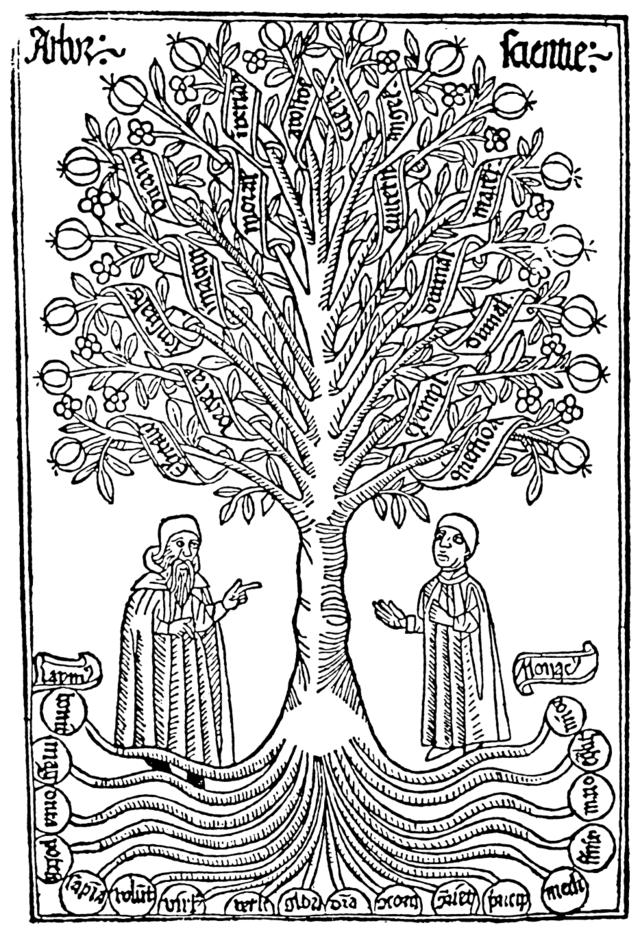
\includegraphics[width=0.5\textwidth]{images/arbor_scientiae.png}
	\caption{L'\textit{Arbor scientiae} de Raymond Lulle}
	\label{fig:arbor_scientiae}
\end{figure}

La visualisation sous forme d'arbre permet d'établir des relations entre les entités en établissant une hiérarchie entre elles. 

\subsubsection{Les cartes}

La cartographie trouve ses racines dans l'Antiquité. Elle est d'abord inventée par des savants comme Anaximandre (vers 500 av. J.-C.) ou Ptolémée (vers 150 ap. J.-C.) pour l'astronomie afin de cartographier le ciel et établir la position des étoiles. 

Au Moyen Age, des cartes représentant Jérusalem à leur centre sont créées sous l'influence du christianisme. Celles-ci sont composées uniquement de l'Europe, de l'Asie et de l'Afrique, l'Amérique n'ayant pas encore découverte par les occidentaux. 

Avec l'impulsion des grandes découvertes, la cartographie évolue avec des projections comme celle de Mercator en 1569\footcite{andryChapitre1Fondements2022}. 

Les cartes sont aussi utilisées dans le contexte militaire. En 1869, Charles Minard réalise la \textit{Carte figurative des pertes successives d'hommes dans l'armée française pendant la campagne de Russie 1812-1813}. A la croisée entre cartographie, chronologie et statistiques, cette dernière représentent les pertes de l'armée de Napoléon Bonaparte durant son aller-retour entre Kaunas et Moscou. L'épaisseur de la ligne diminue au fur et à mesure que le nombre d'hommes baisse. Cette carte montre l'évolution des morts dans l'armée française à cause des maladies, du froid et des escarmouches sur une période où il n'y a pas eu de bataille majeure\footcite{grandjeanIntroductionVisualisationDonnees2015}. 

\begin{figure}[H]
	\centering
	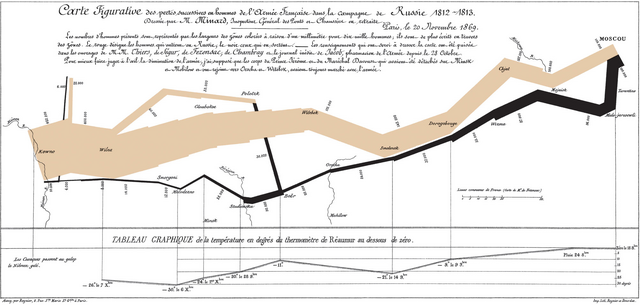
\includegraphics[width=0.8\textwidth]{images/charles_minard.png}
	\caption{\textit{Carte figurative des pertes successives d'hommes dans l'armée française pendant la campagne de Russie 1812-1813} de Charles Minard}
	\label{fig:charles_minard}
\end{figure}

Une carte permet de représenter l'espace, d'y délimiter des territoires, de localiser des éléments et des liens entre ces derniers.
Associée à d'autres domaines comme l'histoire et les statistiques, elle permet de dégager des phénomènes et des irrégularités.

\subsubsection{Les visualisations statistiques}

La visualisation est largement utilisée dans le domaine des statistiques pour explorer les données, en comprendre les tendances et en dégager des conclusions. 

En 1786, William Playfair invente trois types de diagrammes pour des statistiques économiques : 

\begin{itemize}
	\item Le diagramme en ligne
	\item Le diagramme en barre
	\item Le diagramme circulaire 
\end{itemize}

Il est l'auteur de l'\textit{Atlas commercial et politique} qui a pour ambition d'accompagner les hommes politiques à faire des choix rapidement grâce à l'interprétation de diagrammes. 


La \textit{Rose de Nightingale} aussi appelée \textit{visualisation en coxcomb} a été conçue par Florence Nightingale pour représenter les pertes de soldats britanniques pendant la guerre de Crimée (1853-1856). Dans douze secteurs organisés de manière circulaire, la zone bleue montre les décès liés à la maladie et la rouge pour ceux provoqués par des blessures sur le champ de bataille. En observant les résultats de ce graphique, Florence Nightingale en arrive à la conclusion suivante : Les décès sont plus souvent dus à des maladies qu'à des blessures. Grâce à son travail, une réforme est mise en place afin de régler les problèmes d'assainissement dans les casernes\footcite{lagnelBriefOrganisationsElements2021}. 


\begin{figure}[H]
	\centering
	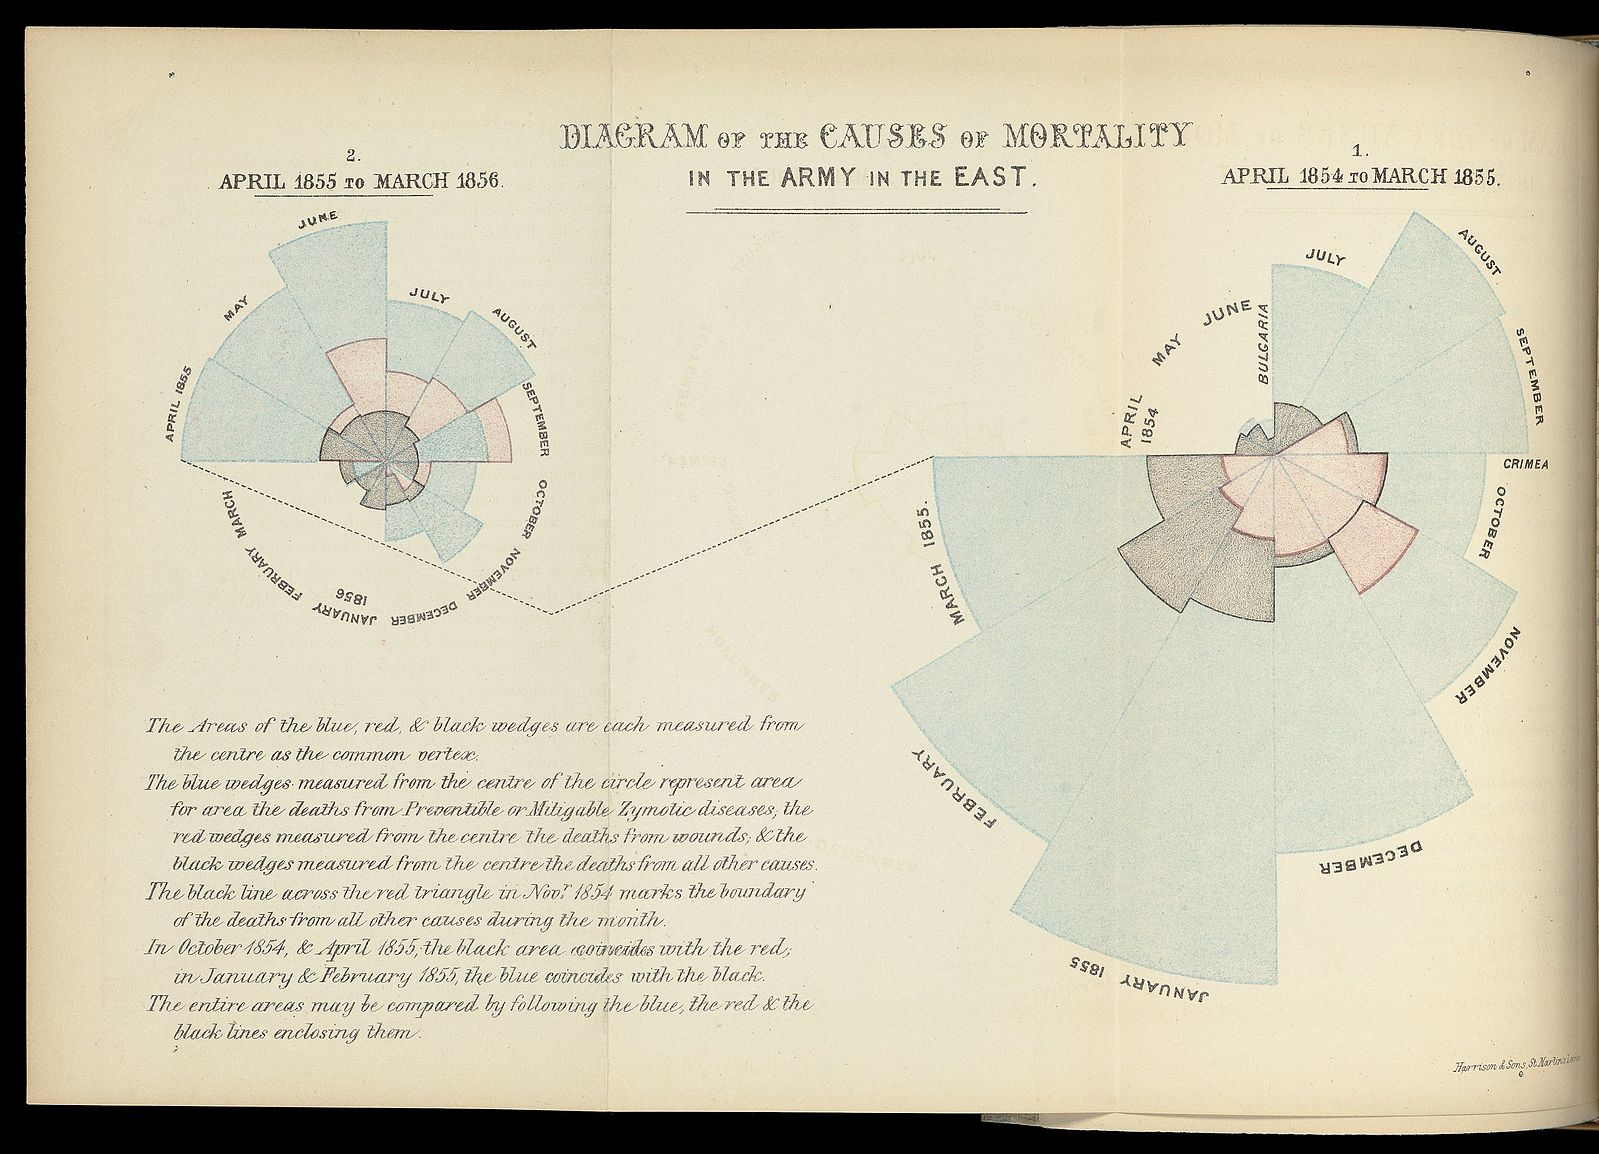
\includegraphics[width=0.8\textwidth]{images/nightingale_rose.jpg}
	\caption{La \textit{Rose de Nightingale}}
	\label{fig:nightingale_rose}
\end{figure}

Ces visualisations influencent depuis longtemps la manière de représenter les données. Cependant, l'arrivée de l'informatique a profondément bouleversé ces pratiques.

\subsection{La visualisation de données à l'ère de l'informatique}

Après une période de déclin nommée par Michael Friendly \og The Modern Dark Ages \fg\footcite{friendlyBriefHistoryData2008}, nous observons une résurgence de la visualisation de données favorisée par l'émergence de l'informatique à partir des années 1950. Au début des années 1980, Edward Tufte publie \textit{The Visual Display of Quantitative Information}\footcite{tufteVisualDisplayQuantitative1983}, un ouvrage qui reste une référence aujourd'hui, pour expliquer comment représenter clairement et efficacement des grands ensembles de données. Ces nouvelles technologies permettent la collecte et le stockage d'une grande quantité de données ainsi que leur traitement et analyse rapide. Cependant, cette masse de données rend leur représentation plus complexe. Les technologies modernes ont permis la création de nouveaux outils comme les tableaux de bord pouvant contenir plusieurs visualisations interactives ou non\footcite{insightsoftwareBreveHistoireVisualisation2023}. Aujourd'hui, le phénomène s'est encore intensifié avec l'avènement du \textit{Big data} et de l'intelligence artificielle qui étendent les options de visualisation\footcite{lagnelAvantPropos2021}.


\subsection{Les différents types de visualisation}

Après avoir retracé l'histoire des visualisations et examiné les enjeux et choix qui y sont liés, nous allons nous concentrer sur les types de visualisations les plus pertinents à utiliser pour l'application AIKON.


La frise chronologique est une visualisation temporelle qui permet de délimiter des périodes et de placer des dates. Elle se présente de manière horizontale ou verticale. Elle peut être interactive afin d'être ludique. Il arrive qu'elle soit associée à d'autres frises ou à une carte. 
Dans le cas de l'application AIKON, associer une frise chronologique à une carte serait particulièrement utile pour contextualiser le corpus.

Les visualisations de la famille des hiérarchies sont adaptées pour représenter les \textit{regions} de l'application AIKON au sein du corpus. 
Le \textit{tree diagram} est une visualisation qui permet de placer des éléments nommés \textit{nœuds} dans une hiérarchie. Le plus haut d'entre eux est appelé \textit{nœud racine} et les liens qui le relient aux autres sont des \textit{branches}. Un nœud peut alors posséder des \textit{frères}, des \textit{parents} et des \textit{enfants}\footcite{BlogDrawTree}. Le \textit{tree diagram} est particulièrement adapté pour montrer les différents niveaux d'un corpus. Le \textit{packed circle}, aussi appelé \textit{circle packing}, présente quant à lui une structure similaire à des poupées russes. Cette visualisation est composée de cercles parents contenant des cercles enfants.
Elle convient mieux aux structures hiérarchiques complexes car elle les rend plus lisibles que la visualisation en \textit{tree diagram}.
De plus, il est possible d'insérer des images au sein des cercles\footcite{lagnelGrandesFamillesRepresentations2021}.

Cependant, les visualisations les plus adaptées pour représenter les \textit{regions pairs} de l'application AIKON sont celles en \textit{networks}.

